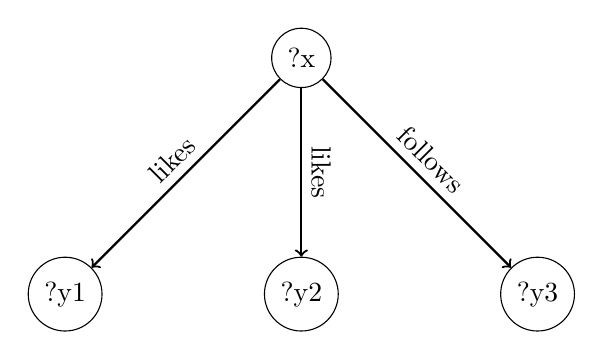
\begin{tikzpicture}[
    node distance=2cm and 3cm,
    node/.style={draw, circle, align=center},
    edge/.style={->, thick},
    slopedlabel/.style={midway, sloped, above, text=black},
]

% Nodes
\node[node] (x) at (0, 0) {?x};
\node[node] (y1) at (-3, -3) {?y1};
\node[node] (y2) at (0, -3) {?y2};
\node[node] (y3) at (3, -3) {?y3};

% Edges
\draw[edge] (x) -- node[slopedlabel] {likes} (y1);
\draw[edge] (x) -- node[slopedlabel] {likes} (y2);
\draw[edge] (x) -- node[slopedlabel] {follows} (y3);

\end{tikzpicture}
